\documentclass{memoir}
\usepackage{mystyle}

\begin{document}

\subsection*{The Matrix of a Transformation}
\setcounter{section}{9}

We have seen that every fin. dim. vector space $V$ is isomorphic to the concrete vector space $\Mat{n}{1}{F}$, where $n = \Dim*[F]{V}$. This alone is a strong statement - it completely characterizes the fin. dim. vector spaces up to isomorphism, which, in the larger context of algebra, is no small feat. But we can do even better. Recall that if $A$ is an $n \times m$ matrix over $F$, then we can think of $A$ as a linear transformation $\Mat{n}{1}{F} \rightarrow \Mat{m}{1}{F}$. It so happens that (1) \emph{every} linear transformation $\Mat{n}{1}{F} \rightarrow \Mat{m}{1}{F}$ can be realized by some matrix, and (2) every linear transformation $V \rightarrow W$ can be thought of as a matrix with respect to given bases.

\begin{dfn}
Let $V$ and $W$ be finite dimensional vector space with ordered bases $\mathcal{B} = \{b_1,\ldots,b_m\} \subseteq V$ and $\mathcal{E} = \{e_1, \ldots, e_n\} \subseteq W$, and let $\varphi : V \rightarrow W$ be a linear transformation. The \emph{matrix} of $\varphi$ with respect to $\mathcal{B}$ and $\mathcal{E}$ is the matrix \[ [\varphi]^\mathcal{B}_\mathcal{E} = \left[\begin{array}{c|c|c|c} [\varphi(b_1)]_\mathcal{E} & [\varphi(b_2)]_\mathcal{E} & \cdots & [\varphi(b_m)]_\mathcal{E} \end{array}\right], \] where $[w]_\mathcal{E}$ is the distinguished isomorphism $[\ast]_\mathcal{E} : W \rightarrow \Mat{n}{1}{F}$ sending $w$ to the $n \times 1$ matrix whose $i$ entry is the $e_i$ coordinate of $w$ with respect to $\mathcal{E}$.
\end{dfn}

To be clear: $[\varphi(b_j)]_{\mathcal{E}}$ is the $m \times 1$ column matrix whose entries are the coordinates of $\varphi(b_j)$ with respect to the ordered basis $\mathcal{E} = \{e_1,\ldots,e_m\}$. To give an example, let \[ \mathcal{B} = \left\{ b_1 = \begin{bmatrix} 1 \\ 0 \end{bmatrix}, b_2 = \begin{bmatrix} 1 \\ 1 \end{bmatrix} \right\}\ \mathrm{and}\ \mathcal{E} = \left\{ e_1 = \begin{bmatrix} 1 \\ 1 \\ 0 \end{bmatrix}, e_2 = \begin{bmatrix} 1 \\ 0 \\ 1 \end{bmatrix}, e_3 = \begin{bmatrix} 0 \\ 0 \\ 1 \end{bmatrix} \right\}. \] Then $\mathcal{B}$ and $\mathcal{E}$ are ordered bases of $\Mat{2}{1}{\mathbb{Q}}$ and $\Mat{3}{1}{\mathbb{Q}}$, respectively (why?). If $\varphi$ is the (unique) linear transformation $\Mat{2}{1}{\mathbb{Q}} \rightarrow \Mat{3}{1}{\mathbb{Q}}$ such that \[ \varphi(b_1) = \begin{bmatrix} 2 \\ 3 \\ 1 \end{bmatrix}\ \mathrm{and}\ \varphi(b_2) = \begin{bmatrix} 4 \\ -7 \\ 5 \end{bmatrix},\] then evidently \[ \varphi(b_1) = 3e_1 + (-1)e_2 + 2e_3 \quad \mathrm{and} \quad \varphi(b_2) = (-7)e_1 + 11e_2 + (-6)e_3. \] So \[ [\varphi]^\mathcal{B}_\mathcal{E} = \begin{bmatrix} 3 & -7 \\ -1 & 11 \\ 2 & -6 \end{bmatrix}. \]

\begin{prp} \mbox{}
\begin{enumerate*}
\item Let $\varphi : V \rightarrow W$ be a linear transformation, where $V$ and $W$ are finite dimensional with ordered bases $\mathcal{B}$ and $\mathcal{E}$, respectively. Then $[\varphi]^\mathcal{B}_\mathcal{E} [v]_\mathcal{B} = [\varphi(v)]_\mathcal{E}$. That is, the following diagram commutes.
\begin{center}
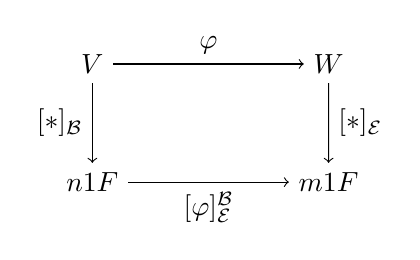
\begin{tikzpicture}[scale=0.3]
  \node (V) at (0,5) {$V$};
  \node (W) at (10,5) {$W$};
  \node (Matn) at (0,0) {$\Mat{n}{1}{F}$};
  \node (Matm) at (10,0) {$\Mat{m}{1}{F}$};
  \draw[->] (V) edge node [above] {$\varphi$} (W);
  \draw[->] (V) edge node [left] {$[\ast]_{\mathcal{B}}$} (Matn);
  \draw[->] (W) edge node [right] {$[\ast]_{\mathcal{E}}$} (Matm);
  \draw[->] (Matn) edge node [below] {$[\varphi]^\mathcal{B}_\mathcal{E}$} (Matm);
\end{tikzpicture}
\end{center}
\item Let $\varphi : V \rightarrow U$ and $\psi : U \rightarrow W$ be linear transformations, where $V$, $U$, and $W$ are finite dimensional with ordered bases $\mathcal{B}$, $\mathcal{K}$, and $\mathcal{E}$, respectively. Then $[\psi]^\mathcal{K}_\mathcal{E} [\varphi]^\mathcal{B}_\mathcal{K} = [\psi\varphi]^\mathcal{B}_\mathcal{E}$.
\end{enumerate*}
\end{prp}

\begin{proof} \mbox{}
\begin{enumerate*}
\item For each $b_j$, write $\varphi(b_j) = \sum_{i=1}^m \mu_{i,j} e_i$. So (by definition) $[\varphi]^\mathcal{B}_\mathcal{E} = [\mu_{i,j}]_{i=1,j=1}^{m,n}$. Given $v \in V$, write $v = \sum_{j=1}^n \alpha_{j,1} b_j$, so that $[v]_\mathcal{B} = [\alpha_{j,1}]_{j=1}^m$. So $[\varphi]^\mathcal{B}_\mathcal{E} [v]_\mathcal{B} = [\sum_{k=1}^n \mu_{i,k} \alpha_{k,1}]_{i=1}^m$. Now
\begin{eqnarray*}
\varphi(v) & = & \sum_{j=1}^n \alpha_{j,1} \varphi(b_j) \\
 & = & \sum_{j=1}^n \alpha_{j,1} \sum_{i=1}^m \mu_{i,j} e_i \\
 & = & \sum_{j=1}^n \sum_{i=1}^m \mu_{i,j} \alpha_{j,1} e_i \\
 & = & \sum_{i=1}^m \left( \sum_{j=1}^m \mu_{i,j} \alpha_{j,1} \right) e_i.
\end{eqnarray*}
By definition, we have \[ \left( [\varphi(v)]_\mathcal{E} \right)_{i,1} = \sum_{j=1}^m \mu_{i,j} \alpha_{j,1} = \left( [\varphi]^\mathcal{B}_\mathcal{E} [v]_\mathcal{B} \right)_{i,1} \] for each $i$, and the conclusion follows.
\item Using (i) we have
\begin{eqnarray*}
[\psi]^\mathcal{K}_\mathcal{E} [\varphi]^\mathcal{B}_\mathcal{K} & = & [\psi]^\mathcal{K}_\mathcal{E} \left[\begin{array}{c|c|c|c} [\varphi(b_1)]_\mathcal{K} & [\varphi(b_2)]_\mathcal{K} & \cdots & [\varphi(b_m)]_\mathcal{K} \end{array}\right] \\
 & = & \left[\begin{array}{c|c|c|c} [\psi]^\mathcal{K}_\mathcal{E} [\varphi(b_1)]_\mathcal{K} & [\psi]^\mathcal{K}_\mathcal{E} [\varphi(b_2)]_\mathcal{K} & \cdots & [\psi]^\mathcal{K}_\mathcal{E} [\varphi(b_m)]_\mathcal{K} \end{array}\right] \\
 & = & \left[\begin{array}{c|c|c|c} [(\psi\varphi)(b_1)]_\mathcal{E} & [(\psi\varphi)(b_2)]_\mathcal{E} & \cdots & [(\psi\varphi)(b_m)]_\mathcal{E} \end{array}\right] \\
 & = & [\psi\varphi]^\mathcal{B}_\mathcal{E} \qedhere
\end{eqnarray*}
\end{enumerate*}
\end{proof}

\begin{dfn}
Let $V$ be a finite dimensional vector space and suppose $\mathcal{B} = \{b_1,\ldots,b_n\}$ and $\mathcal{E} = \{e_1,\ldots,e_n\}$ are ordered bases of $V$. The matrix $[1]^\mathcal{B}_\mathcal{E}$ is called the \emph{change of basis matrix} from $\mathcal{B}$ to $\mathcal{E}$.
\end{dfn}

\begin{prp} \mbox{}
\begin{enumerate*}
\item The map $[\ast]^\mathcal{B}_\mathcal{E} : \Hom[F]{V}{W} \rightarrow \Mat{n}{m}{F}$ is an isomorphism of vector spaces.
\item The map $[\ast]^\mathcal{B}_\mathcal{B} : \End*[F]{V} \rightarrow \Mat{n}{n}{F}$ is an isomorphism of rings.
\end{enumerate*}
\end{prp}

\begin{proof} \mbox{}
\begin{enumerate*}
\item Recall that it suffices to show that $[\ast]$ preserves addition and scalar multiplication and that $[\ast]$ is bijective.
\begin{itemize*}
\item We have 
\begin{eqnarray*}
[\varphi + \psi]^\mathcal{B}_\mathcal{E} [v]_\mathcal{B} & = & [(\varphi+\psi)(v)]_\mathcal{E} = [\varphi(v) + \psi(v)]_\mathcal{E} = [\varphi(v)]_\mathcal{E} + [\psi(v)]_\mathcal{E} \\
 & = & [\varphi]^\mathcal{B}_\mathcal{E}[v]_\mathcal{B} + [\psi]^\mathcal{B}_\mathcal{E}[v]_\mathcal{B} = ([\varphi]^\mathcal{B}_\mathcal{E} + [\psi]^\mathcal{B}_\mathcal{E})[v]_\mathcal{B}
\end{eqnarray*}
for all $v \in V$, so that $[\varphi+\psi]^\mathcal{B}_\mathcal{E} = [\varphi]^\mathcal{B}_\mathcal{E} + [\psi]^\mathcal{B}_\mathcal{E}$.
\item We have \[ [\alpha\varphi]^\mathcal{B}_\mathcal{E} [v]_\mathcal{B} = [\alpha\varphi(v)]_\mathcal{E} = \alpha [\varphi(v)]_\mathcal{E} = \alpha [\varphi]^\mathcal{B}_\mathcal{E} [v]_\mathcal{B} \] so that $[\alpha\varphi]^\mathcal{B}_\mathcal{E} = \alpha [\varphi]^\mathcal{B}_\mathcal{E}$.
\item If $[\varphi]^\mathcal{B}_\mathcal{E}$ is the zero matrix, then we have $\varphi(b_j) = 0$ for all $b_j \in \mathcal{B}$. So in fact $\varphi = 0$. Since $\kernel*{[\ast]} = 0$, the map $[\ast]$ is injective.
\item Let $A \in \Mat{n}{m}{F}$, and define $f : \mathcal{B} \rightarrow W$ by $f(b_j) = \sum_{i=1}^n A_{i,j} e_i$. (That is, let $\varphi(b_j)$ be the linear combination of the $\mathcal{E}$ whose coefficients are the $j$th column of the matrix $A$.) Now $f$ lifts to a linear transformation $\varphi : V \rightarrow W$, and by definition $[\varphi]^\mathcal{B}_\mathcal{E} = A$. So $[\ast]$ is surjective.
\end{itemize*}
\item In the light of (i), it suffices to show that $[\ast]$ preserves multiplication and 1. But $[\varphi\psi] = [\varphi][\psi]$ is precisely the content of 9.2(ii), and certainly $[1]^\mathcal{B}_\mathcal{B} = I_n$. \qedhere
\end{enumerate*}
\end{proof}

So far we have shown that every vector space is isomorphic to a vector space of column matrices, and that under this isomorphism every linear transformation can be realized by a matrix. We thus have two points of view from which to study finite dimensional vector spaces: the abstract language of vector spaces and the concrete language of matrices. Neither point of view is better than the other, and each brings unique insights. For instance, proofs written from the abstract point of view are typically more succinct and, once we get used to it, easier to find, because they can ignore obfuscating details and see the essence of a problem. The lifting property of bases is one example of this. On the other hand, matrices are nice, concrete, computational objects, which are easy to represent in a computer and with which we can give the abstract theory real, computational interpretations.

This dichotomy, by the way, between the abstract and the concrete is a very powerful and pervasive paradigm in modern mathematics and has yielded much fruit.

\end{document}